%!TEX root = ../Thesis.tex
\section*{Anhang}
\addcontentsline{toc}{section}{Anhang}
\fancyhead[R]{Anhang}

\anhangsverzeichnis

\anhang{Tabellen}
\subanhang{Auswertungsmatrix alter Vermögensverzeichnis Dialog}
\begin{minipage}{\textwidth}
    \begin{figure}[H]
      \centering
      \includegraphics[width=390px]{img/Auswertungsmatrix_Alter_Dialog.PNG}
      \caption*{\textbf{Quelle:} Eigene Darstellung}
      \label{fig:auswertungsmatrixAlterDialog}
    \end{figure}
\end{minipage}

\subanhang{Datentabelle zu Interaktionen im alten Dialog}
\label{sec:datentabelleAlterDialog}
\begin{figure}[H]
    \begin{minipage}[H]{1\textwidth}	
        \centering
         \includegraphics[angle=90, width=0.54\textwidth]{img/Datentabelle_Alter_Dialog}
        \label{fig:datentabelleAlterDialog}
    \end{minipage}
    \source{Eigene Darstellung}
\end{figure}

\subanhang{Datentabelle zu Interaktionen im neuen Dialog}
\label{sec:datentabelleNeuerDialog}
\begin{figure}[H]
    \begin{minipage}[H]{1\textwidth}	
        \centering
         \includegraphics[angle=90, width=0.54\textwidth]{img/Datentabelle_Neuer_Dialog}
        \label{fig:datentabelleNeuerDialog}
    \end{minipage}
    \source{Eigene Darstellung}
\end{figure}

\anhang{Diagramme}
\subanhang{Ablauf Zwangsvollstreckung}
\label{sec:ablaufZwangsvollstreckung}
\begin{figure}[H]
\centering
    \begin{minipage}[H]{1\textwidth}
        \includegraphics[width=1\textwidth]{img/Zwangsvollstreckung_Prozess}
        \source{Eigene Darstellung}
        \label{fig:ablaufZwangsvollstreckung}
    \end{minipage}
\end{figure}

\subanhang{Relative Häufigkeit von Veränderungen (Verteilung)}
\label{sec:verteilungVeraenderungen}
\begin{figure}[H]
    \begin{minipage}[H]{1\textwidth} % Breite, z.B. 1\textwidth		
        \centering
        \includegraphics[angle=90, width=0.5\textwidth]{img/Verteilung_Veraenderungen}
        \label{fig:verteilungVeraenderungen}
    \end{minipage}
    \source{Eigene Darstellung} % Quelle
\end{figure}

\subanhang{ERM UIDataCollector}
\label{sec:ermUIDataCollector}
\begin{figure}[H]
    \begin{minipage}[H]{1\textwidth}
        \centering
        \includegraphics[width=.8\textwidth]{img/ERM_UIDataCollector}
        \caption*{\textbf{Quelle:} Eigene Darstellung}
        \label{fig:ermUIDataCollector}
    \end{minipage}
\end{figure}


\anhang{Dokumente}
\subanhang{Beispielformular Vermögensverzeichnis}
\label{sec:beispielVermoegensverzeichnisFormular}
\begin{minipage}{\textwidth}
  \centering
  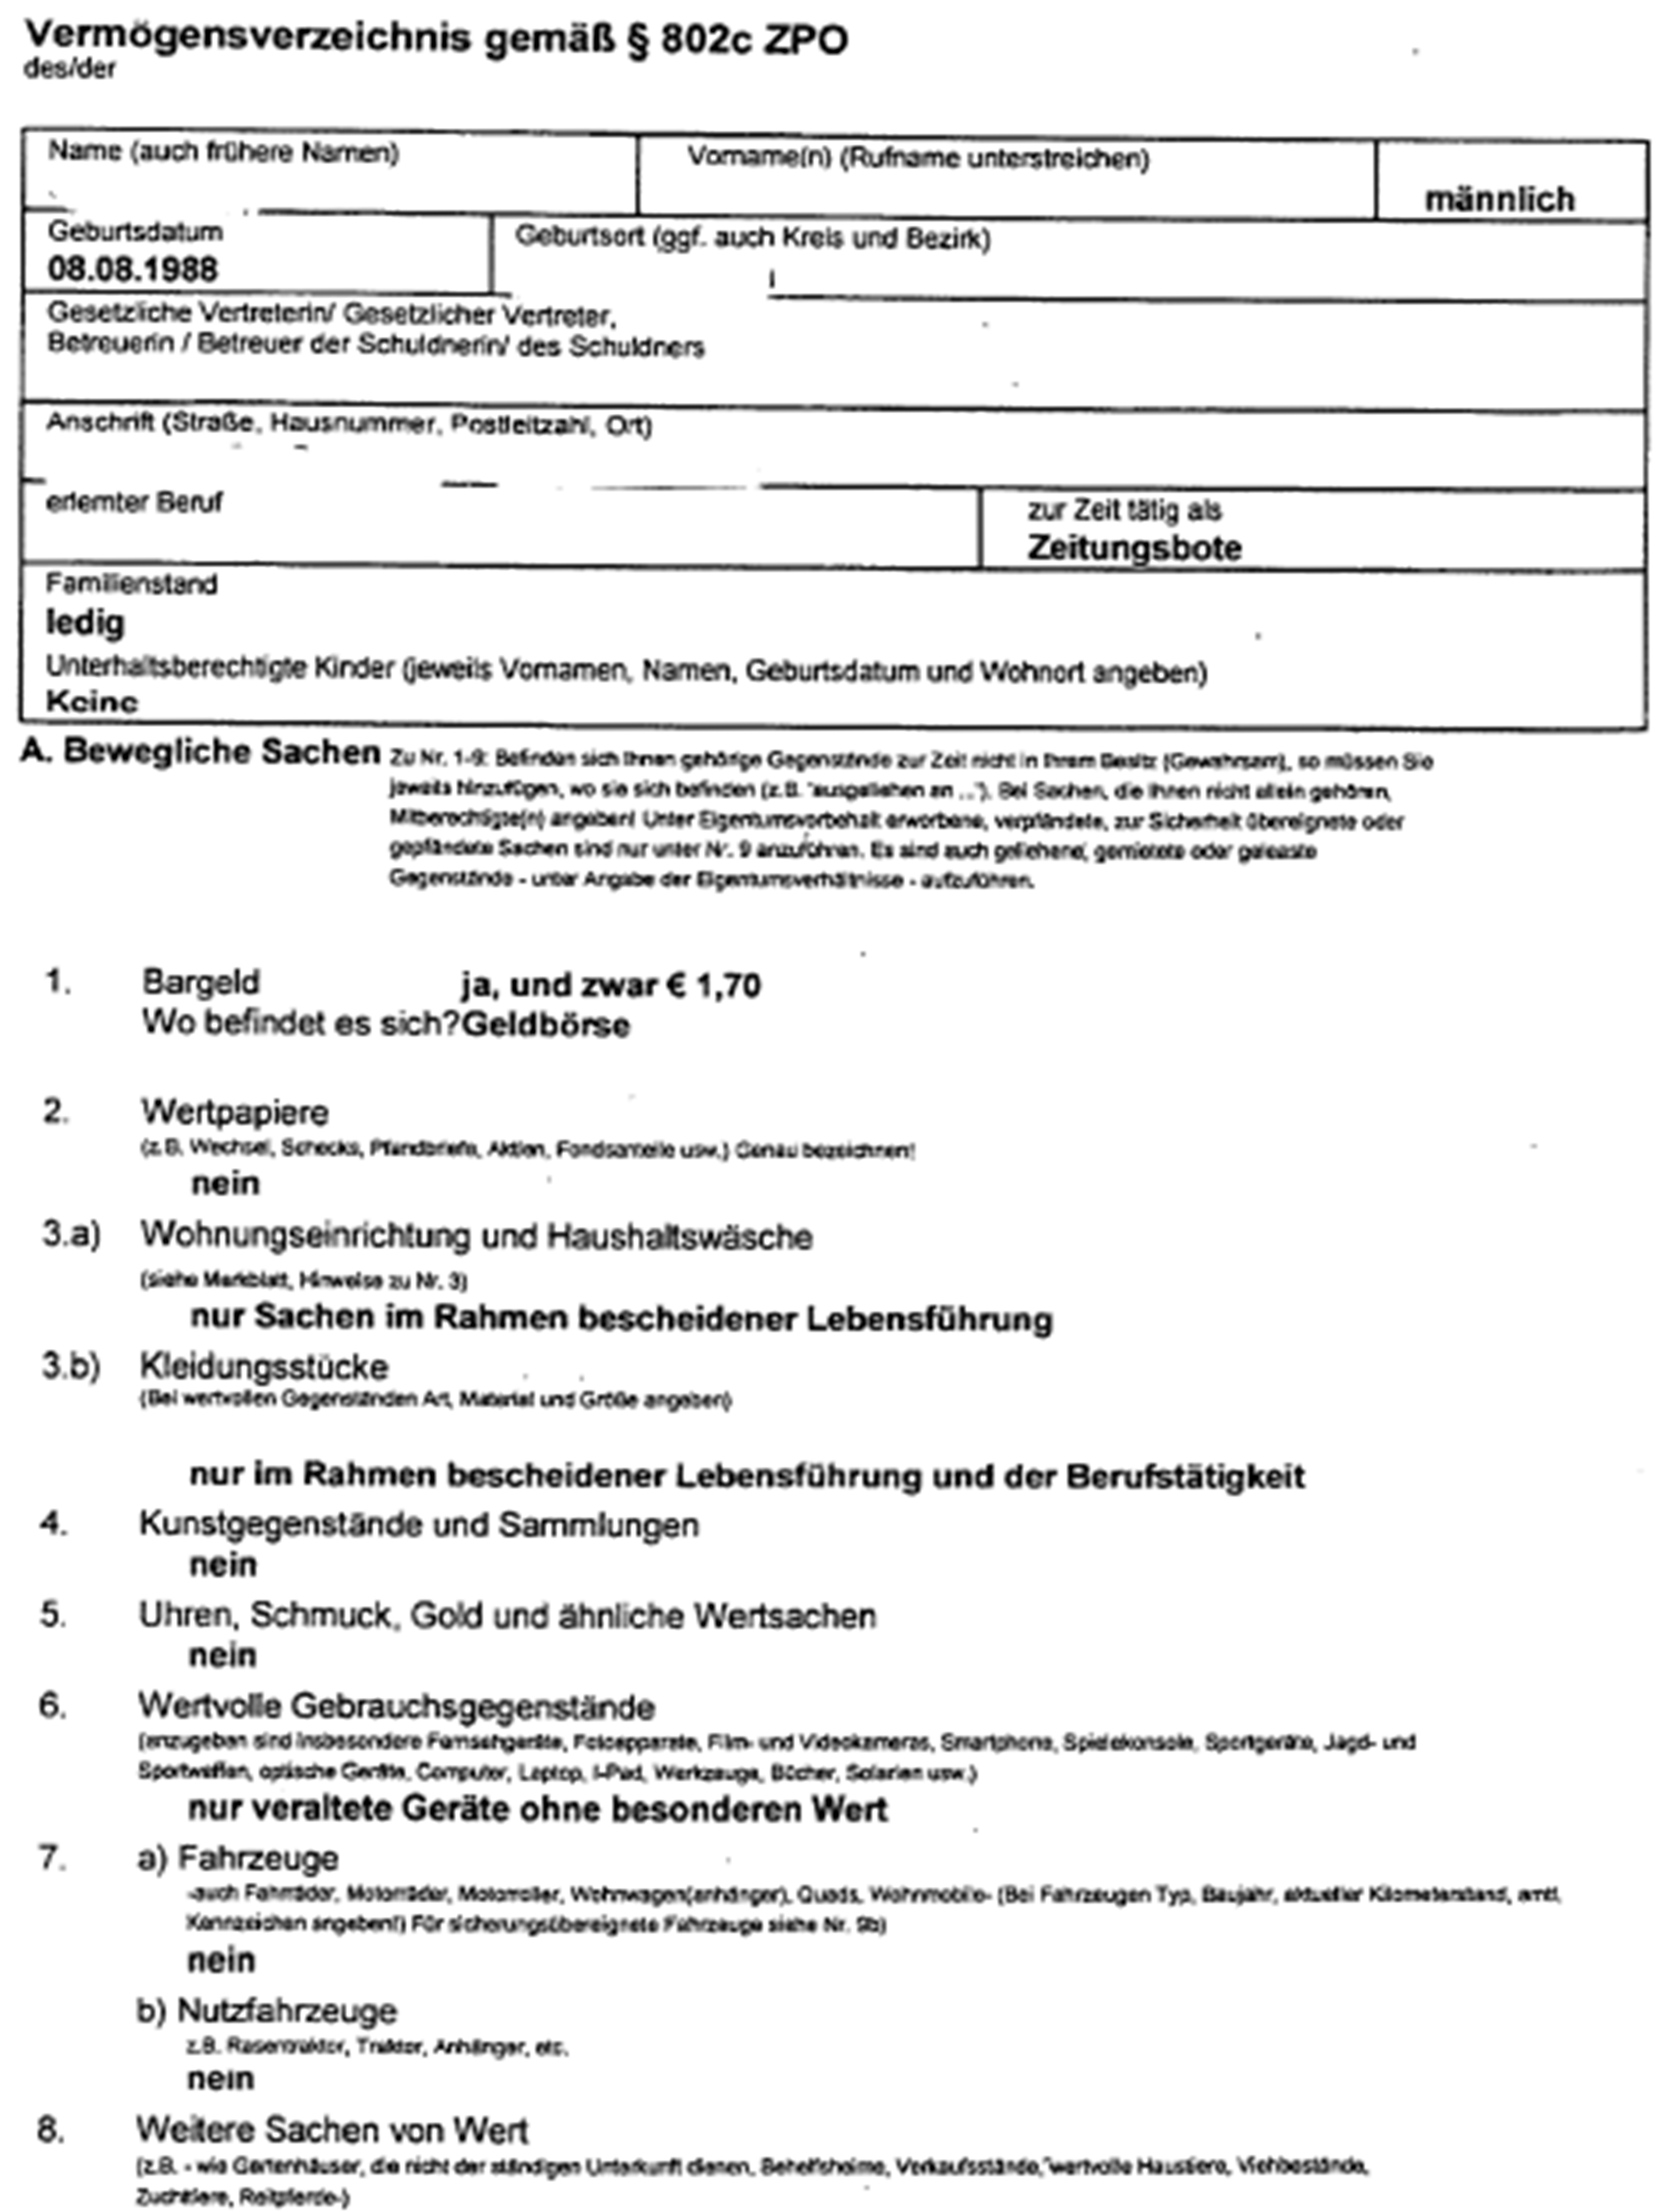
\includegraphics[scale=0.91]{img/VVFormular_1.png}
\end{minipage}

\bigskip\noindent
\begin{minipage}{\textwidth}
  \centering
  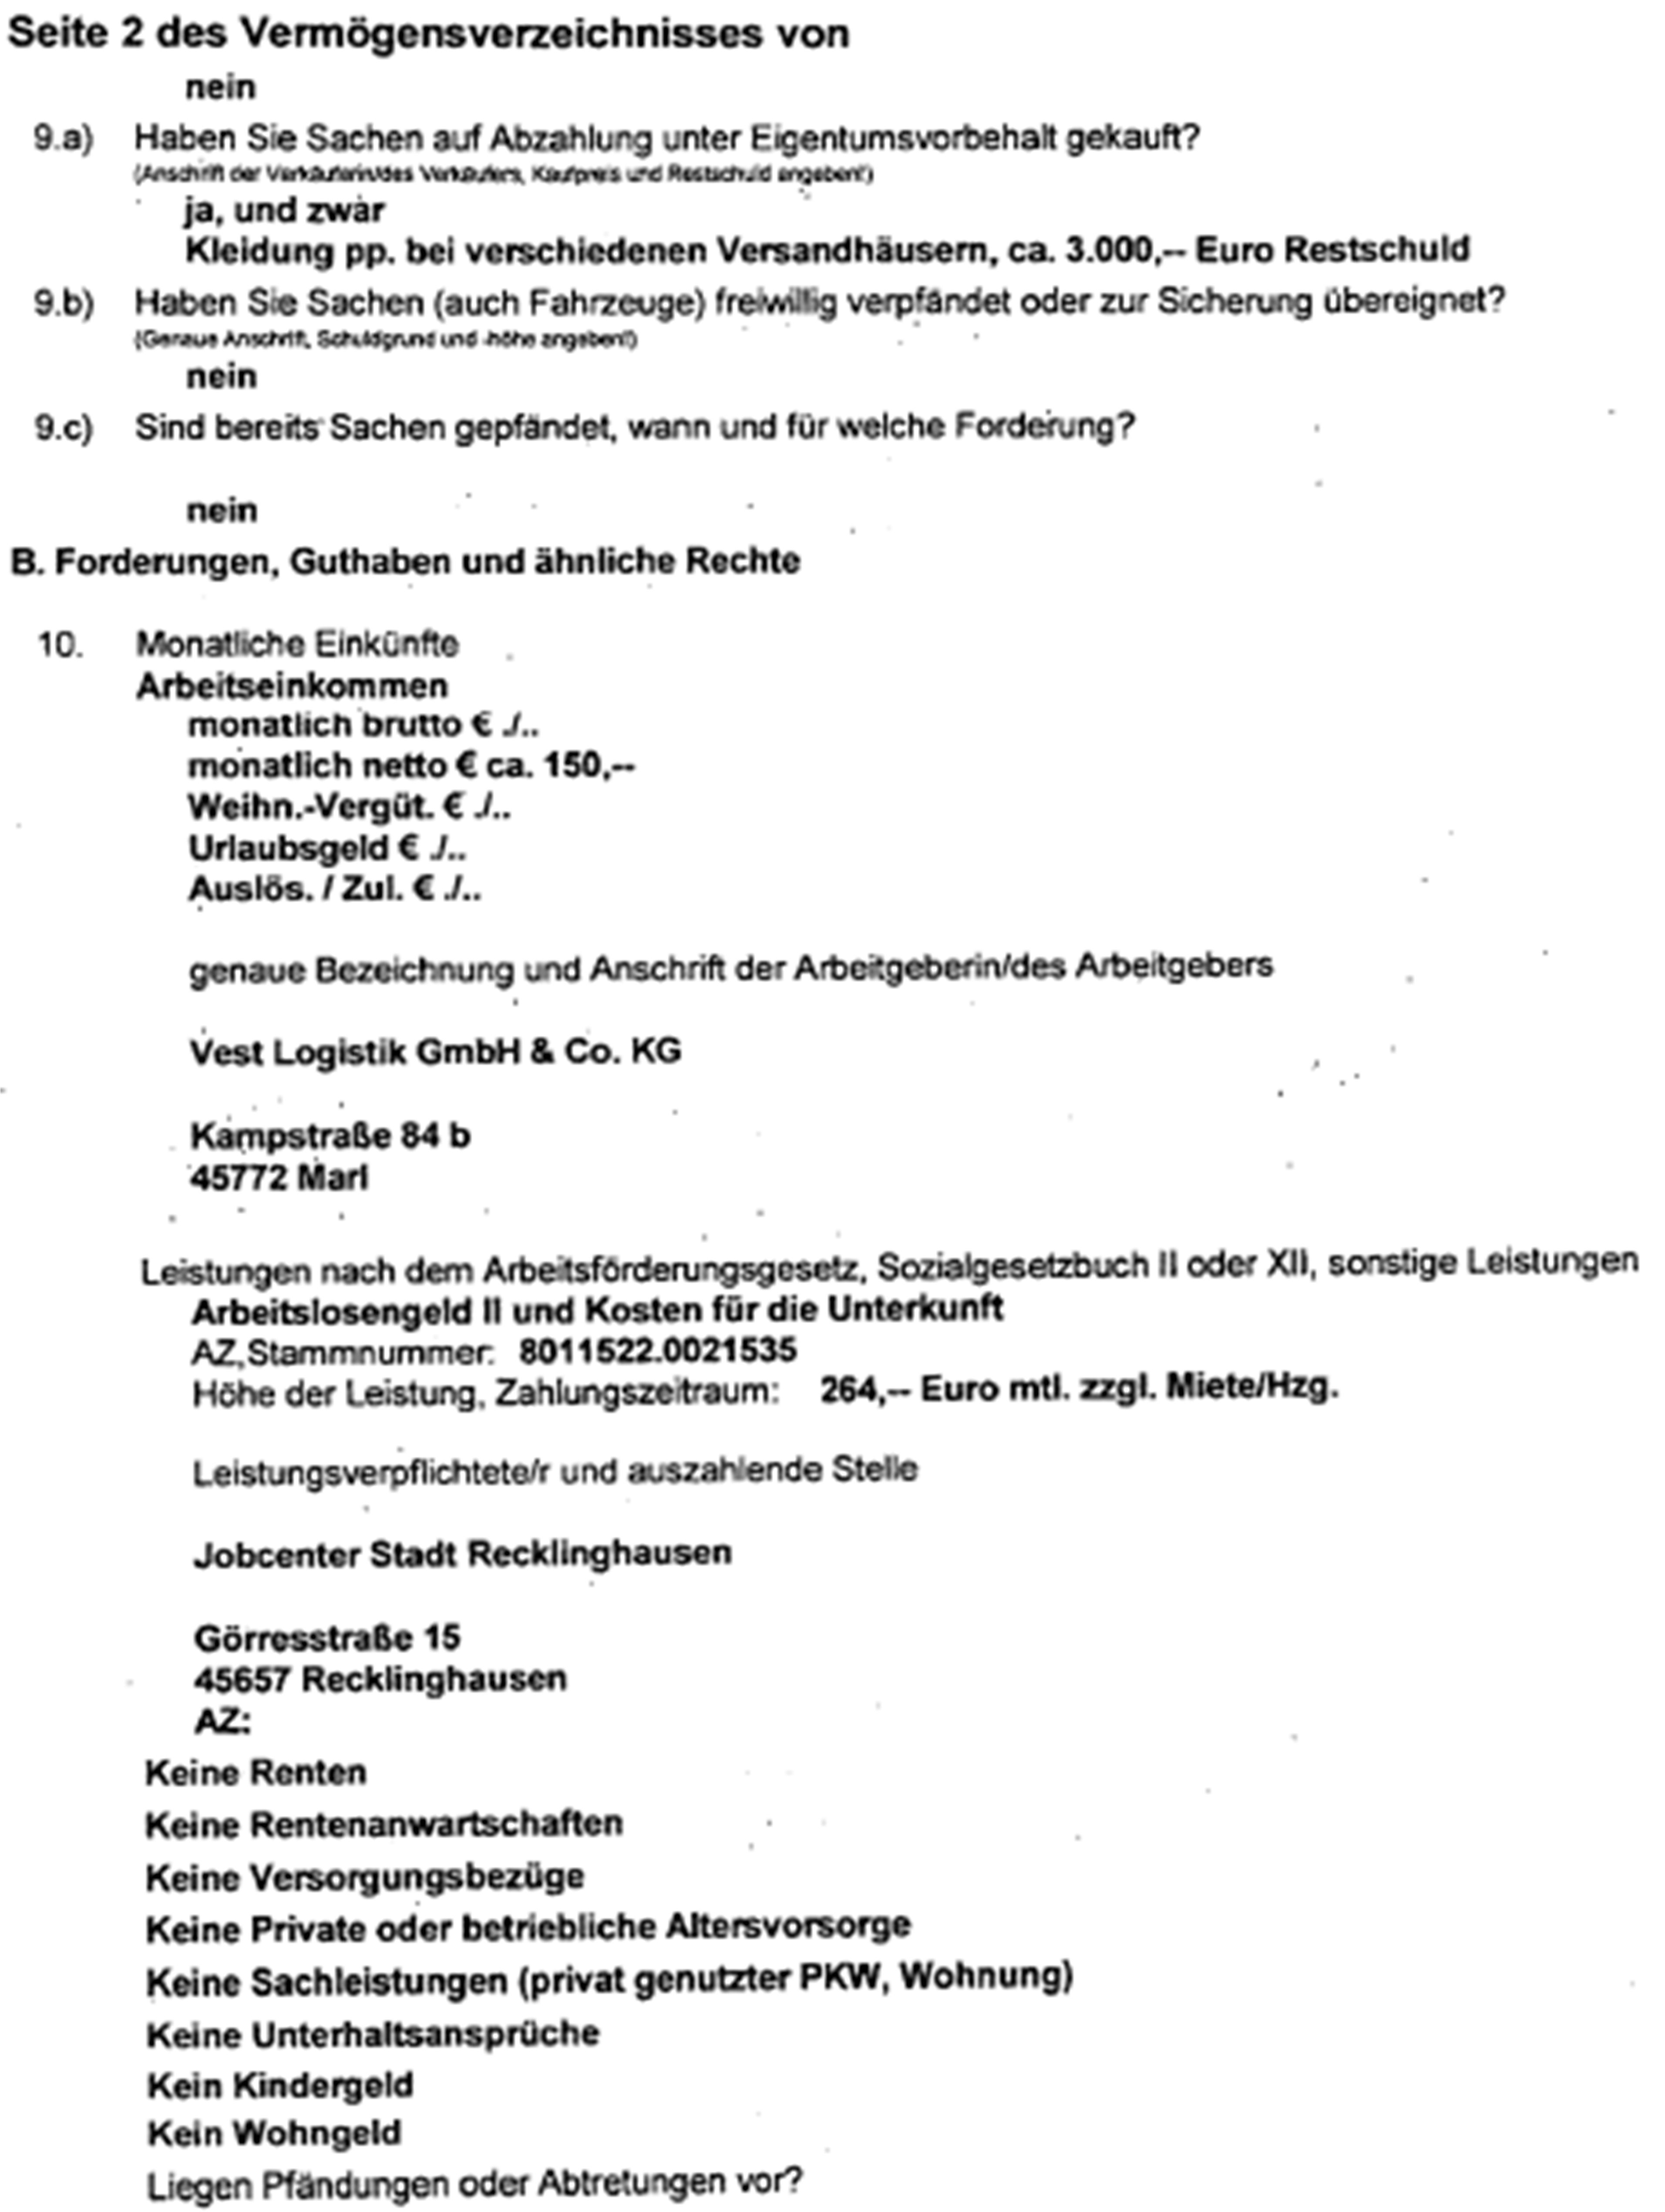
\includegraphics{img/VVFormular_2.png}
\end{minipage}

\bigskip\noindent
\begin{minipage}{\textwidth}
  \centering
  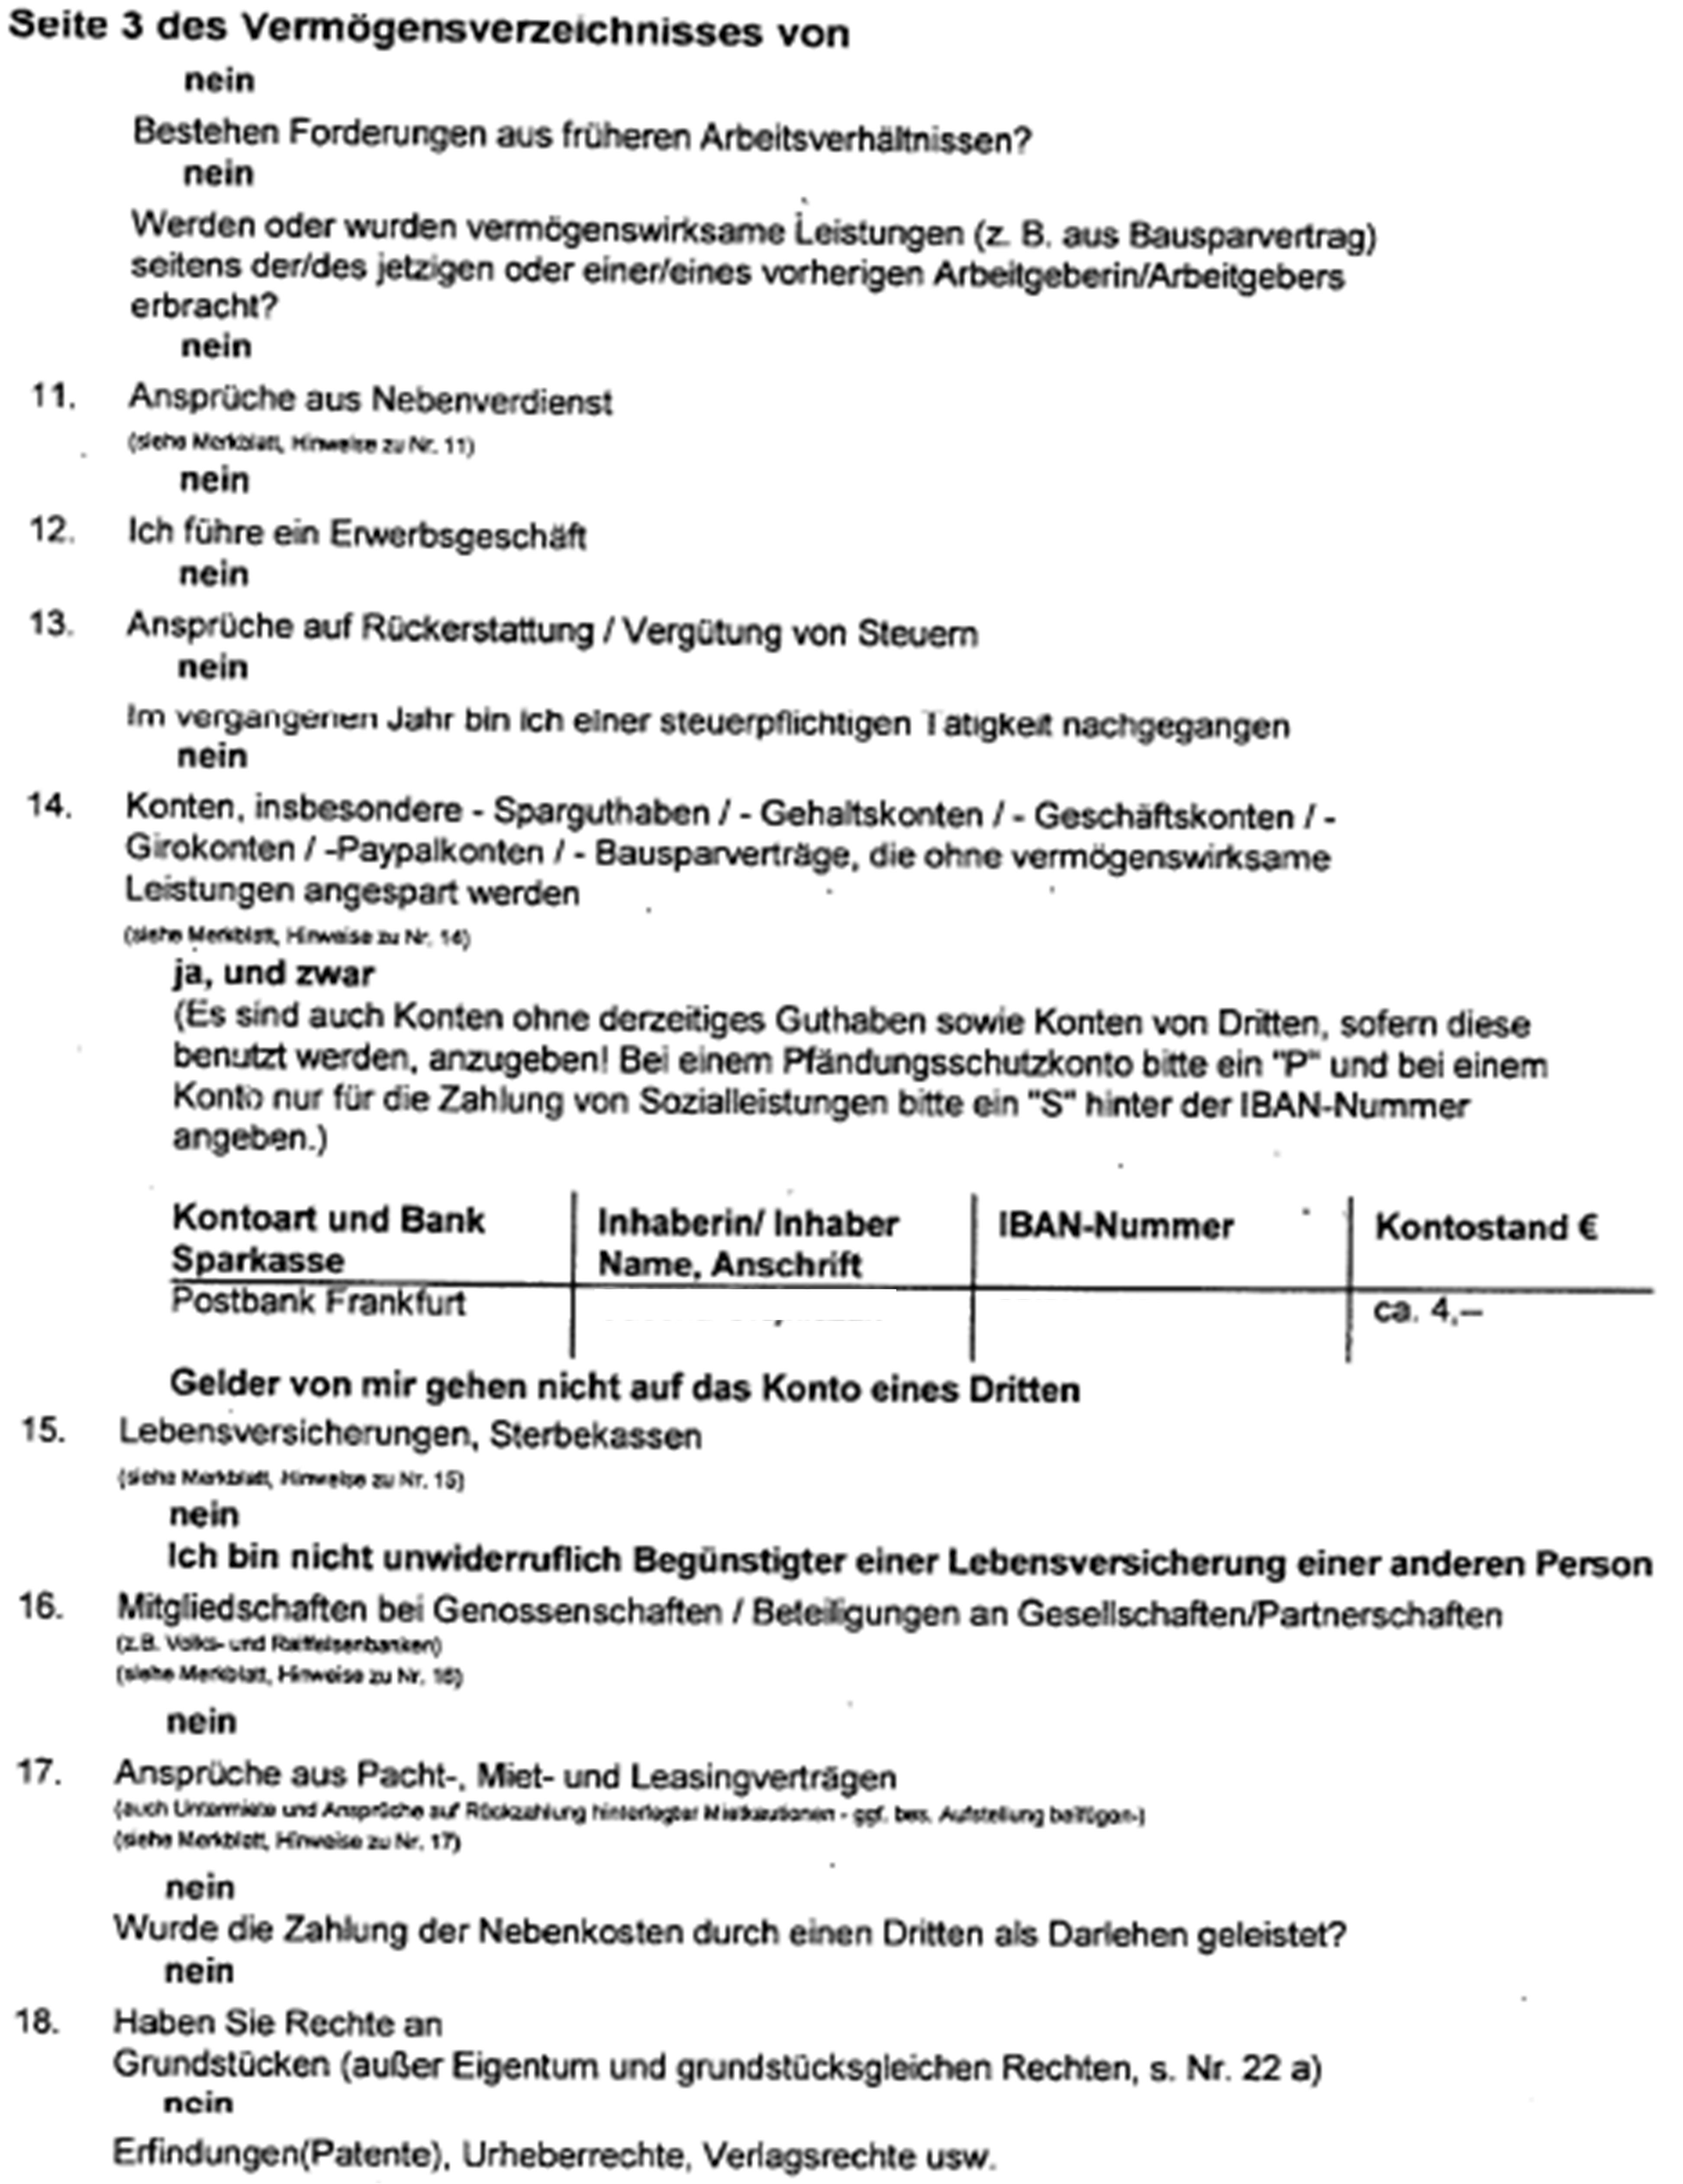
\includegraphics{img/VVFormular_3.png}
\end{minipage}

\bigskip\noindent
\begin{minipage}{\textwidth}
  \centering
  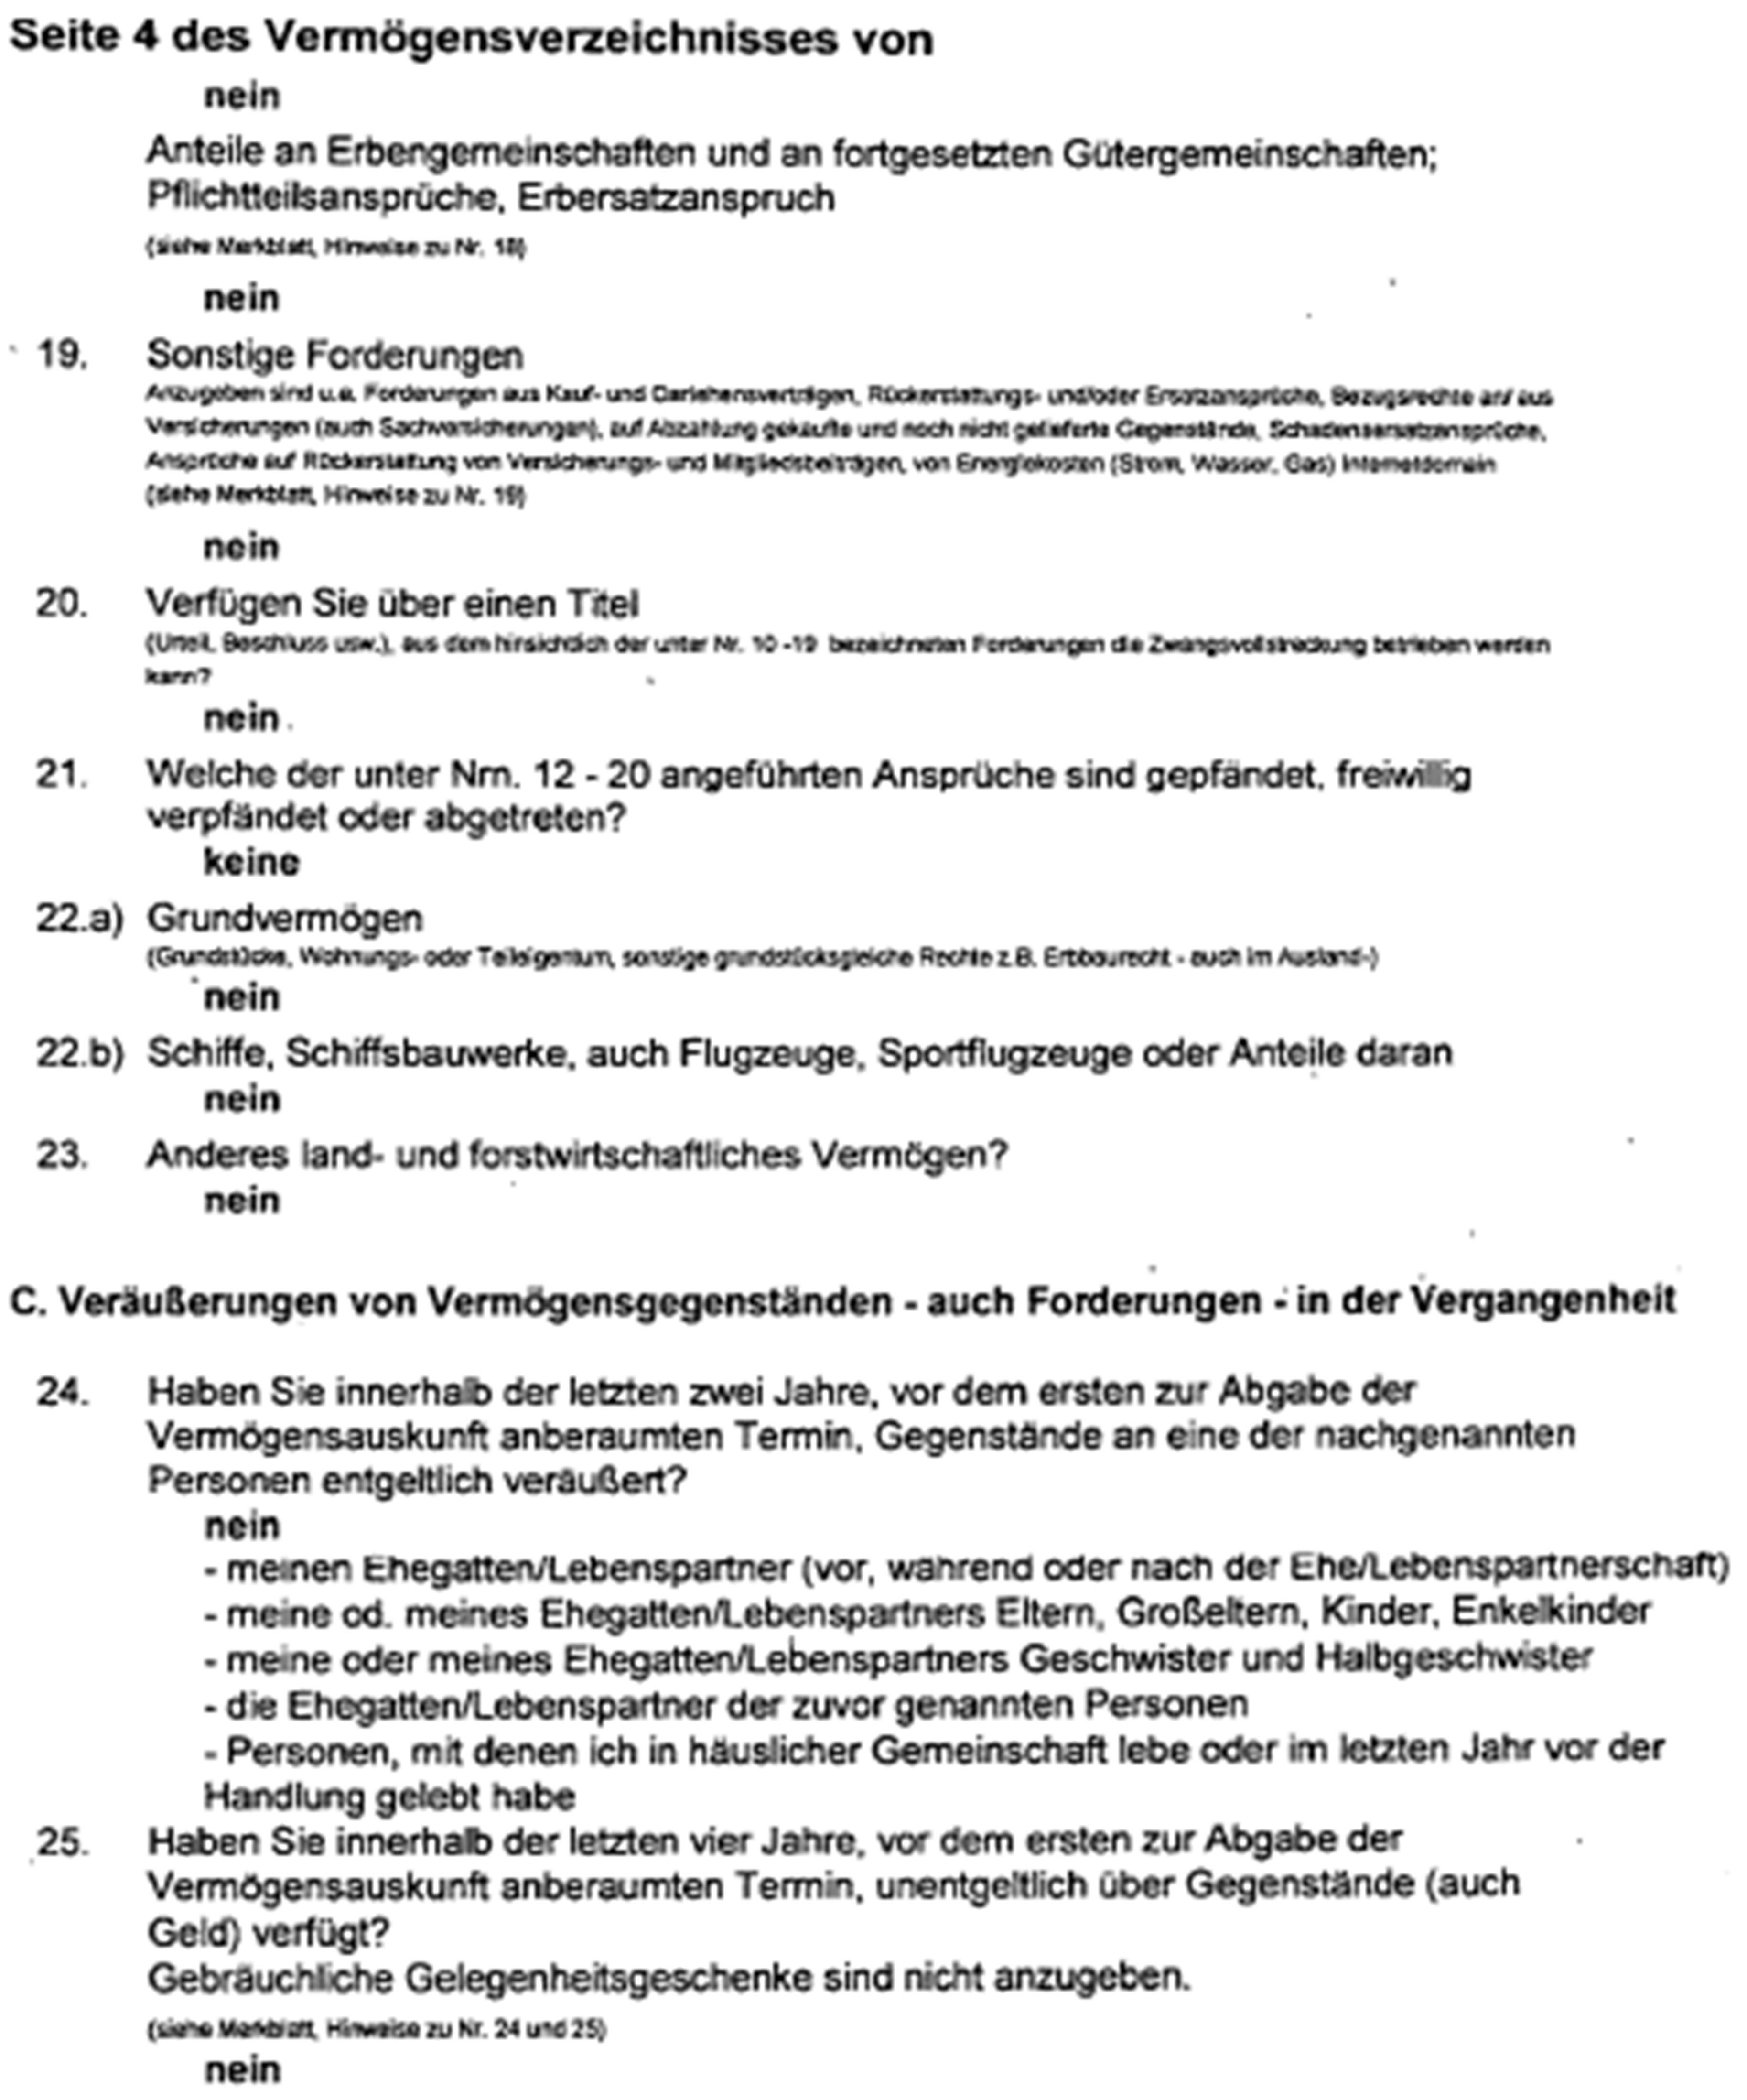
\includegraphics{img/VVFormular_4.png}
\end{minipage}

\let\cleardoublepage\clearpage
\subanhang{ISO9241-10 Fragebogen}
\label{sec:ISOFragebogen}
\bigskip\noindent
\begin{minipage}{\textwidth}
  \centering
  \includegraphics[scale=0.97]{img/ISO9241-10Fragebogen_S1.PNG}
\end{minipage}

\bigskip\noindent
\begin{minipage}{\textwidth}
  \centering
  \includegraphics{img/ISO9241-10Fragebogen_S2.PNG}
\end{minipage}

\bigskip\noindent
\begin{minipage}{\textwidth}
  \centering
  \includegraphics{img/ISO9241-10Fragebogen_S3.PNG}
\end{minipage}

\bigskip\noindent
\begin{minipage}{\textwidth}
  \centering
  \includegraphics{img/ISO9241-10Fragebogen_S4.PNG}
\end{minipage}

\bigskip\noindent
\begin{minipage}{\textwidth}
  \centering
  \includegraphics{img/ISO9241-10Fragebogen_S5.PNG}
\end{minipage}

\bigskip\noindent
\begin{minipage}{\textwidth}
  \centering
  \includegraphics{img/ISO9241-10Fragebogen_S6.PNG}
\end{minipage}

\bigskip\noindent
\begin{minipage}{\textwidth}
  \centering
  \includegraphics{img/ISO9241-10Fragebogen_S7.PNG}
\end{minipage}